
\chapter{Introduction} % Main chapter title


%----------------------------------------------------------------------------------------
%	SECTION 1
%----------------------------------------------------------------------------------------
\vspace{-1cm}
\section{The biology of cancer}

\label{Intro-biology} 
Cancer was the second cause of death worldwide, with almost 10 million deaths, in 2018 \cite{Bray2018} and could in a near future become the leading cause \cite{Dagenais2020}. The disease can affect different parts of the body, although some tissues are more frequently altered than others.  Lung cancer, on which the work described in this manuscript will focus, is one of the most common cancers and the deadliest according to the 2018 GLOBOCAN database (a project of the \gls{IARC} providing worldwide cancer statistics)  \cite{Bray2018}. Cancer is a complex disease that is highly controlled by the genome \cite{Stratton2009,Wishart2015}. It originates from normal cells whose genetic information has been altered. Those alterations can result from endogenous processes as well as from exogenous processes like environmental exposures and lifestyle \cite{Eggert2011,Luch2005}. As a result of these alterations, tumor cells have acquired specific capabilities that allow them to grow in an uncontrolled way as opposed to normal cells. These capabilities are referred to as the hallmarks of cancer and are listed in Figure \ref{fig:intro_hallmarks} \cite{Hanahan2011}.
\begin{figure}[H]
    \centering
    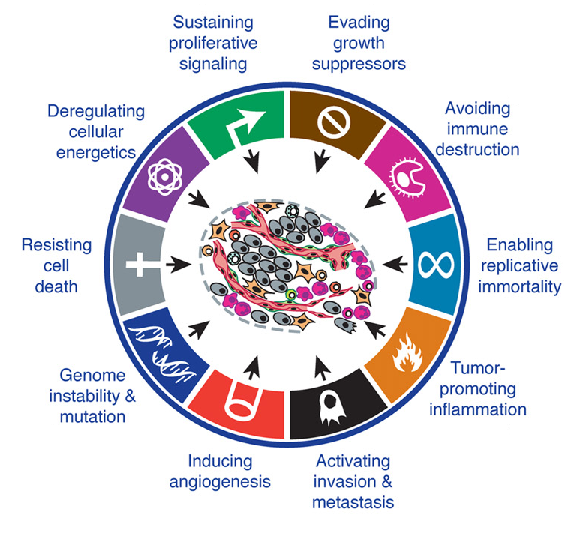
\includegraphics[width=0.55\textwidth]{Figures/Intro/hallmarks.pdf}
    \caption[The hallmarks of cancer]{\textbf{The hallmarks of cancer}. From Hanahan \textit{et al.} \cite{Hanahan2011}}
    \label{fig:intro_hallmarks}
\end{figure}
The first part of the introduction describes how genomic changes can influence cancer development and how the technological advances in the genomics area have enabled to shed lights on the mechanisms involved. 

\subsection{The central dogma of molecular biology}
%good videaos: https://www.youtube.com/watch?v=J3HVVi2k2No   https://www.khanacademy.org/test-prep/mcat/biomolecules/amino-acids-and-proteins1/v/central-dogma-of-molecular-biology-2
%\textit{"DNA makes RNA makes protein"}, Marshall Niremberg, Nobel price in Physiology and Medicine in 1968. \\

%Cancer complexity: from Genome to Proteome
At the beginning of the 19th century, Avery and colleagues isolated and identified the \gls{DNA} as the molecule constituting our chromosomes, defined previously as carriers of our hereditary material by Thomas Morgan \cite{Avery1944,Morgan}. In 1953, Watson and Crick proposed a new structure for the \gls*{DNA} molecule, the double helix structure \cite{Watson1953} (See Figure \ref{fig:intro_fig1}A). Five years later, Francis Crick formulates how the information contained in the sequence of nucleic acids is processed to produce the proteins needed by our cells in what is called the central dogma of molecular biology (Figure \ref{fig:intro_fig1}B-C). 
\begin{figure}[H]
    \centering
    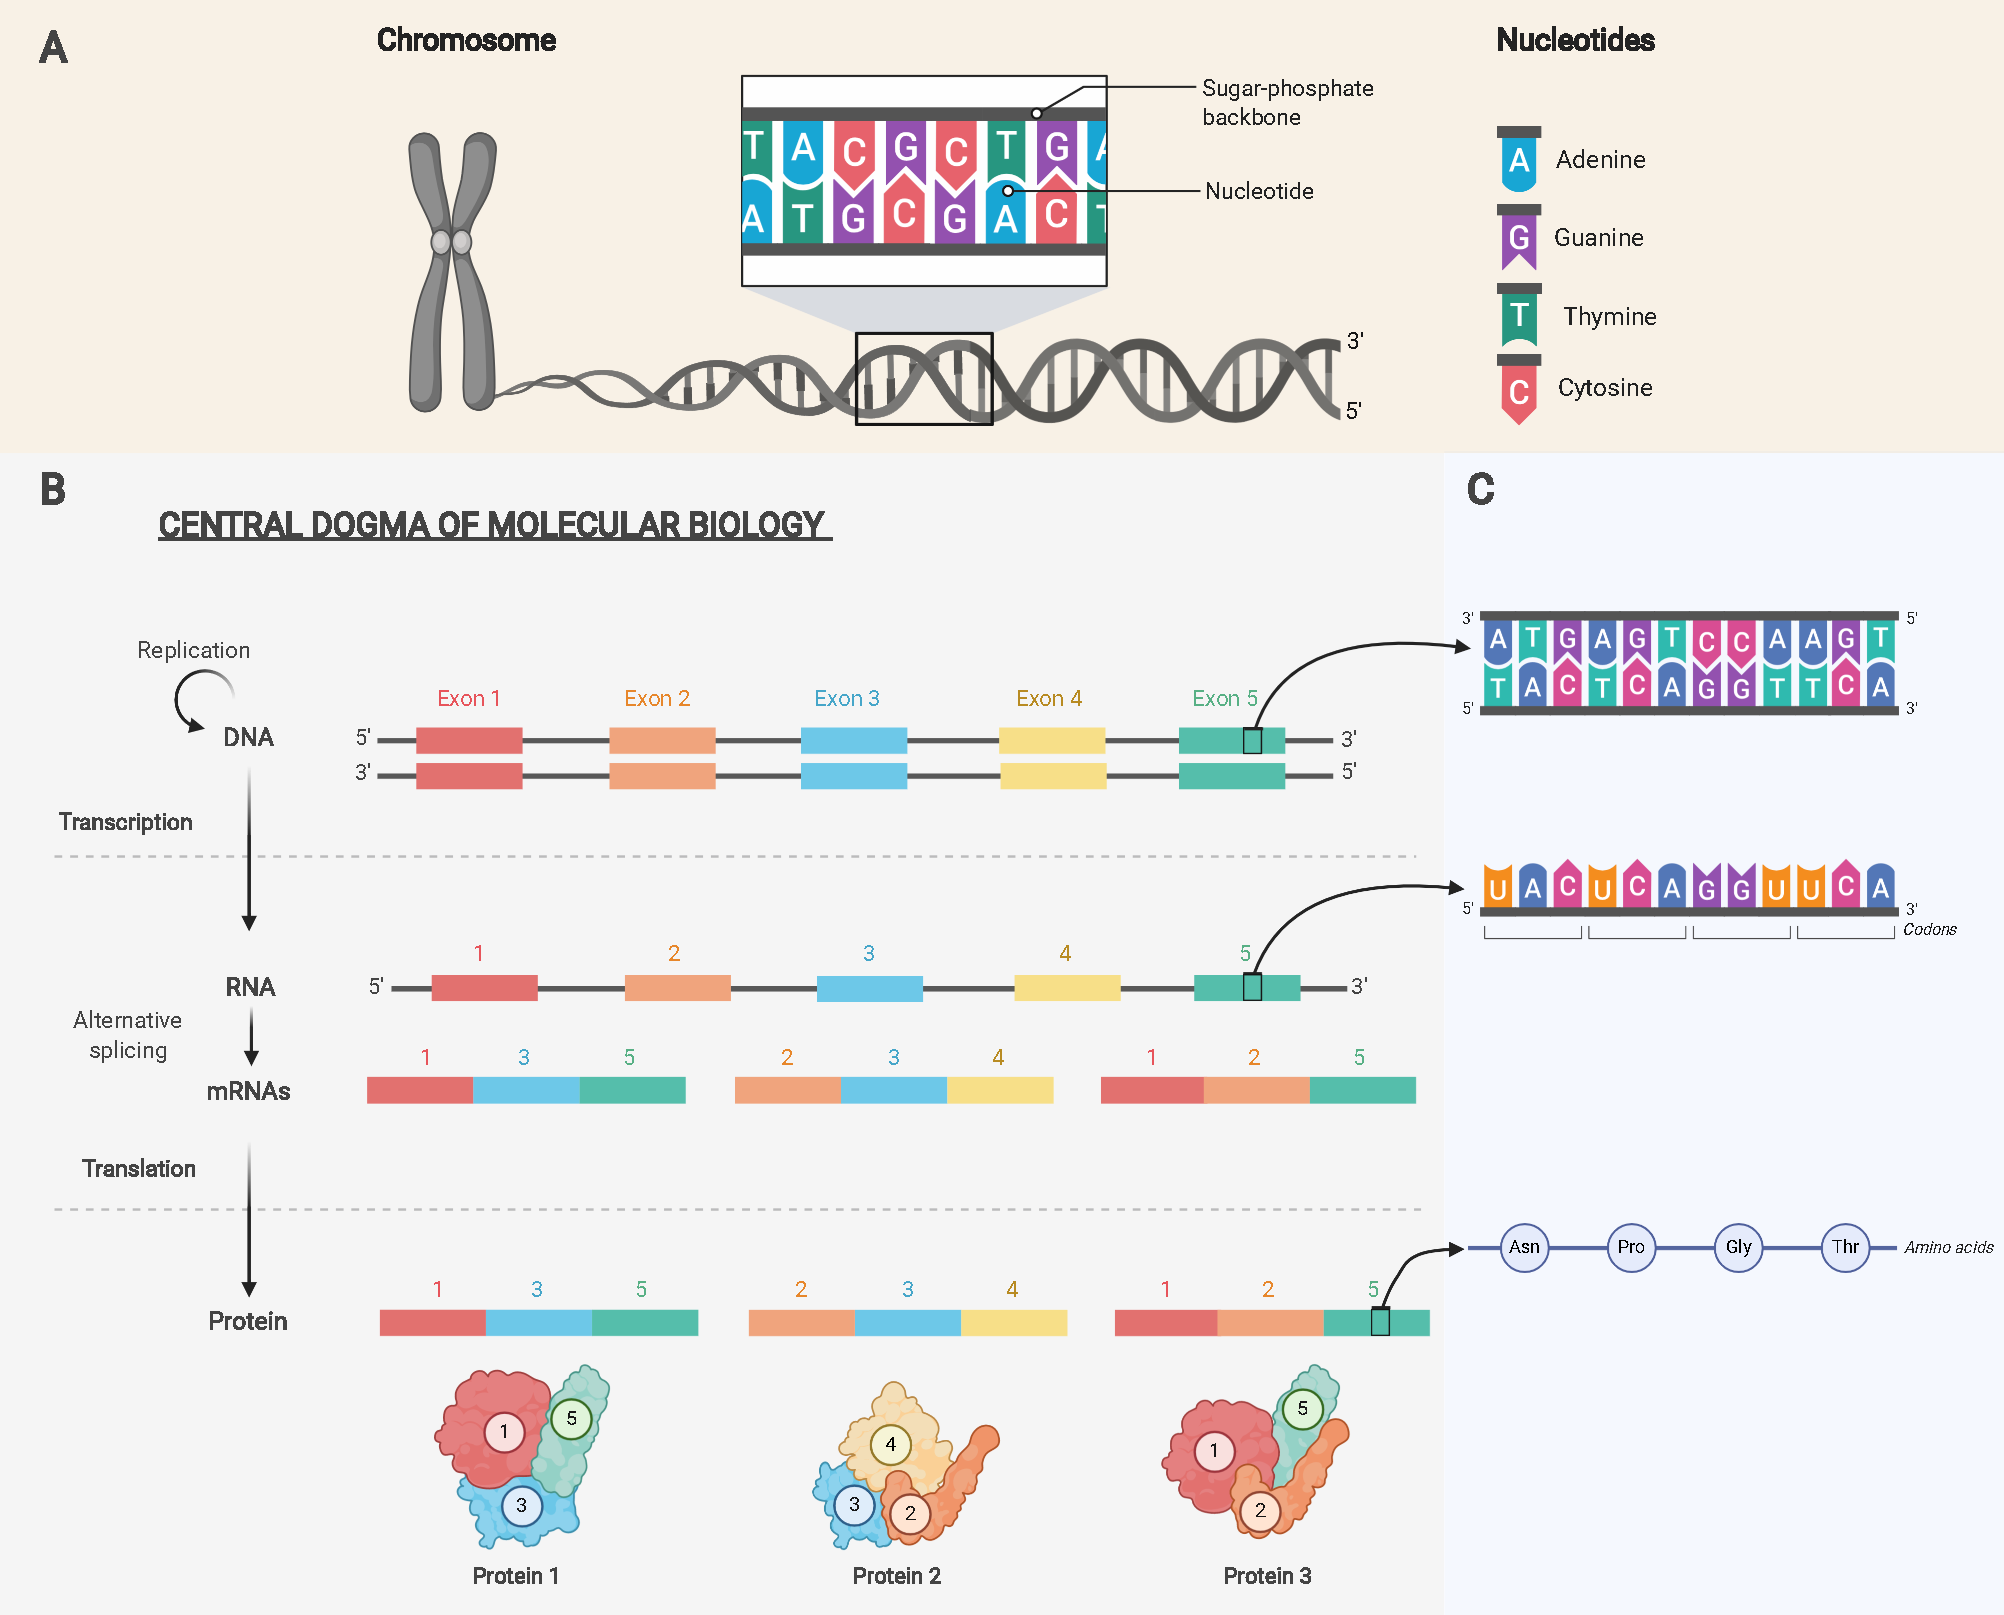
\includegraphics[width=0.95\textwidth]{Figures/Intro/Fig_1.pdf}
    \caption[The DNA molecule and the central dogma of molecular biology]{\textbf{The \gls*{DNA} molecule and the central dogma of molecular biology}. A) The structure of \gls*{DNA}: the double helix molecule is composed of two complementary strands of nucleotides. B) Representation of the steps described by the central dogma of molecular biology. C) Illustration of the molecules resulting from the central dogma transfers at a higher resolution. Created with \href{https://biorender.com/}{BioRender.com}}
    \label{fig:intro_fig1}
\end{figure}
Three main transfers are described by the central dogma: replication, transcription and translation (See Figure \ref{fig:intro_fig1}B). During replication, the \gls*{DNA} molecule is duplicated to provide the needed information to progeny cells. Through the two other steps, the information contained in \gls*{DNA} is used to generate proteins. Firstly, the process of transcription consists in reading the \gls*{DNA} sequence to synthesize a single-stranded molecule of the same length, the \gls{RNA}. During translation, the transcribed molecule is then read using a reading frame of three nucleotides that form what is called a codon encoding for one amino acid, the unit of a protein (See Figure \ref{fig:intro_fig1}C). Note that the genetic code is redundant; multiple codons can encode an amino acid. The conversion of the information encoded in our genes to functional gene products like proteins is referred to as gene expression.

%more complexity
Since the statement of the central dogma, other mechanisms have been identified as determinant for the expression of a protein. Firstly, the \gls*{RNA} molecule resulting from the transcription process, containing regions coding for the final amino acids sequence (exons) and non-coding regions (introns), is actually a \gls{pre-mRNAs}. The step transforming precursor \gls*{RNA} to mature \gls{mRNAs} is called alternative splicing and consists in truncating intronic regions and joining different exons together (See Figure \ref{fig:intro_fig1}B). Hence, one pre-mRNA can lead to multiple \gls{mRNAs} that are then transported outside of the nucleus to be translated into different proteins. While around 20,000 genes are described, much more proteins are generated as a result of alternative splicing.

% regulatory elements
Although all of our cells share the same genetic information and follow the same dogma, it is known that cells in distinct tissues differentiate and do not express the same proteins, at the same time. Such differences can be explained by the fact that several regulatory processes control gene expression levels.
Firstly, genes transcription is dependent on transcription factors that represent around 7\% of the genes \cite{Weinberg2014}. They specifically bind to control regions of genes,  provide or prevent access to the \gls*{DNA} and can control multiple genes \cite{Weinberg2014}. The fact that genes, for example the transcription factors, can influence multiple genes and thus multiple possibly unrelated phenotypes is referred to as pleiotropy.
After transcription, \gls{mRNAs} can also be regulated through other \gls*{RNA} molecules, like the \gls{miRNAs}, that can degrade \gls{mRNAs}. %Those micro-RNAs might explain why the mRNA expression levels do not always correlate with protein expression levels. 
% epigenetic events
Besides, differences in gene expression can be controlled via non-genetic mechanisms like epigenetic processes, including histone modifications and \gls*{DNA} methylation. Histones are proteins around which the \gls*{DNA} is wrapped and hence control \gls*{DNA} accessibility (Figure \ref{fig:intro_fig2}). For example, histone phosphorylation leads to the condensation of the chromatin and inhibits gene expression \cite{Weinberg2014}.
\gls*{DNA} methylation consists in the addition of a methyl group to cytosine nucleotides located in \gls{CpG} dinucleotides sites (cytosine followed by a guanine nucleotide). Such positions are not homogeneously distributed across the genome and are more frequently observed in what is called \gls{CpG} islands, themselves mainly observed in regulatory regions of genes, the promoters. It has been observed that the methylation of \gls{CpG} sites in promoters can repress gene expression while methylation of positions in the gene body positively correlates with gene expression \cite{Ma2013a}. 
\begin{figure}[H]
    \centering
    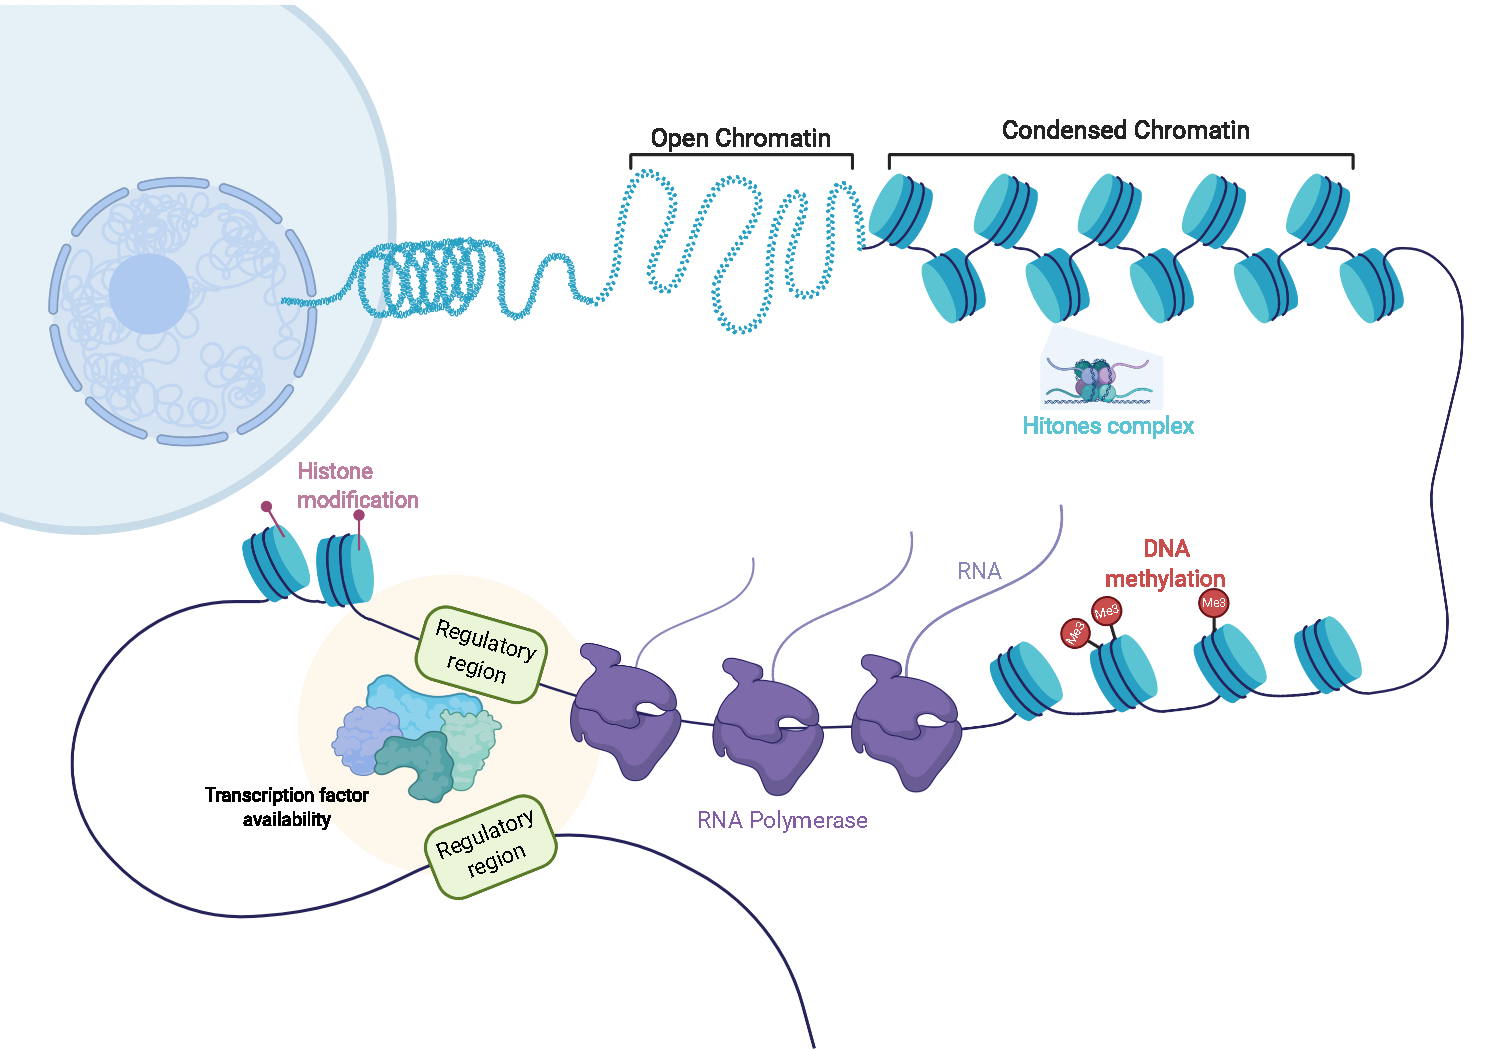
\includegraphics[width=0.8\textwidth]{Figures/Intro/transcription_regulation.pdf}
    \caption[Regulation of transcription]{\textbf{Regulation of transcription}. The figure represents different configurations of \gls*{DNA} packaging. The \gls*{DNA} molecule is wrapped around histones proteins that themselves are gathered in complexes called nucleosomes. This packaging forms the chromatin structure. This structure can be more or less compact (open versus condensed chromatin), which is influencing gene expression. When the chromatin is open, transcription factors can access the \gls*{DNA} molecule, and \gls*{RNA} polymerases can initiate the transcription. Note that the structure of the chromatin can be influenced by histones modifications and \gls*{DNA} methylation events. Created with \href{https://biorender.com/}{BioRender.com}}
    \label{fig:intro_fig2}
\end{figure}
Finally, post-translational events like enzymatic modifications of proteins or protein cleavage can occur and increase the number of proteins that can be generated in human cells, hence adding an additional layer of complexity.
% Impact on gene expression. For multiple tasks in the cells, translation, repairing DNA, replication, DNA must be open (euchromatin).
%house keeping genes vs tissue specific genes

%These elements highlight the complexity of the molecular mechanisms. There are even mechanisms that goes against the central dogma, for example the reverse transcription: we can go back to the DNA level; other example, non coding RNA that skip the step of translation.

As such, the numerous steps of transferring the \gls*{DNA} sequence information to proteins reflect the complexity behind protein expression. Any of these steps can be disrupted and result in altered molecules and proteins, leading to cancer development.  

\subsection{Cancer: a genomic disease}

%The previous section suggests that maintaining DNA integrity is critical to allow our cells to function properly. However, 
Our \gls*{DNA} continuously undergoes diverse alterations %altered what is called mutations 
and their accumulation over time can cause cancer. Researchers started to investigate the role of genomes in cancer at the end of the 19th century. In 1890, David von Hansemann, by observing cancer cell division under a microscope, identified for the first time abnormal chromosomes. This observation, among others, led Theodor Boveri 20 years later to suggest that cancer was a consequence of alterations in our inherited \gls*{DNA} \cite{Stratton2009}. His hypothesis was supported in the mid 20th century by the identification of a recurrent alteration resulting in a peculiar chromosome 22 (the Philadelphia chromosome), in \gls{CML}.
While those alterations have been observed at the chromosomal level, genomes can be impacted by a multitude of alterations detectable at a lower resolution, the modification of one nucleotide in the \gls*{DNA} sequence being the lowest resolution. 

At any position of the genome, the nucleotides might vary from an individual to another as well as between cells of an individual; those variations are called \gls{SNVs}. Also, larger events like nucleotides \gls{indels} of up to 1,000 bases and structural variations (chromosomal rearrangements or large \gls{indels}) can alter the \gls*{DNA} sequence. All of these genomic changes are called mutations.
\begin{figure}[H]
    \centering
    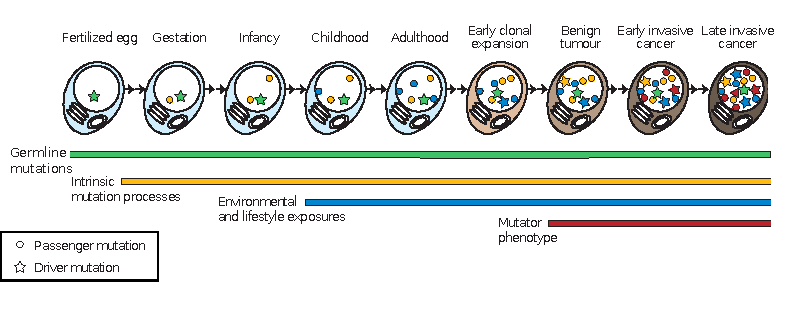
\includegraphics[width=1\textwidth]{Figures/Intro/Fig_mutation_over_life.pdf}
    \caption[The timing of somatic mutations acquisition]{\textbf{The timing of somatic mutations acquisition}. Mutations can be inherited at birth (germline mutations, in green) or acquired during life course (somatic mutations, in yellow, blue and red). They can have little to no impact (passenger mutations represented by circles) or confer an advantage to the cell (driver mutations represented by stars). Adapted from Stratton \textit{et al. } \cite{Stratton2009}}
    \label{fig:intro_fig3}
\end{figure}
%germline vs somatic alterations
Mutations can occur at different moments in life (See Figure \ref{fig:intro_fig3}). Some mutations are inherited at birth since they are present in the germ line cells (sperm and egg) transmitted by parents to the offspring. They are called germline mutations and are found in all the cells of an individual, normal cells as well as tumor cells. 
Such mutations are observed at different frequencies in different populations and are called \gls{SNP}s. %Note though that the notion of SNPs is usually extended to any germline variation. 
Another category of mutations can also be found in all cells of the body even if they were not transmitted by our parents, if they occur early in life during the development, at gestation. They are called \textit{de novo} mutations. Finally, the rest of the mutations found in humans are acquired later in life as a result of errors in the \gls*{DNA} maintenance or exogenous damages (See next section). Those mutations occur in cells outside the germ line and are called the somatic mutations. 
%In a human genome, each mutation type is not expected at the same frequency, a germline mutation is expected every 1,000 bases when somatic mutations every 1,000,000 bases approximately depending on the cancer type \cite{Alexandrov2013}. 

%impact of mutations
Also, whether they are germline or somatic, mutations can have different impacts. Most mutations have, due to the redundancy of the genetic code, little to no impact on the genes encoded around them, they are the passenger mutations \cite{Vogelstein2013}. Others though alter the gene product and confer a selective advantage to the cell, \textit{e.g.} a faster proliferation or a better survival in comparison to neighbour cells \cite{Stratton2009}. Those mutations are called driver mutations as they are thought to contribute to “driving the carcinogenic process” and are preserved by positive selection. In 2018, the Cancer Gene Census described more than 700 driver genes (genes carrying driver mutations). Among them, 90\% were associated with somatic mutations and 20\% contained germline mutations \cite{Sondka2018,CancerGeneCensus}. Generally, two types of driver genes exist, oncogenes and \gls{TSG}. 
Oncogenes are genes whose functions are to promote cell growth, proliferation or inhibit apoptosis and usually result from a gain of function. A mutation in an oncogene can thus lead to a deregulation of one of these processes, hence resulting in uncontrolled proliferation and cancer. The first mutation identified as causing cancer was discovered in 1982 by Reddy \textit{et al.} and was activating an oncogene named \textit{HRAS} \cite{Reddy1982}. Besides mutations, other processes like over-expression of genes via amplification or chromosomal translocations can activate this category of genes. 
%Some mutations can alter the gene product because they truncate the protein, some can impact the levels of expression (mention structural variants and copy number changes).  
In contrast to oncogenes, \gls{TSG}s are refraining cellular growth and proliferation and are often referred to as the "gatekeepers" genes. Mutations in \gls{TSG}s tend to result in a loss of function; the latter genes are inactivated, and their negative regulation of cell proliferation is cancelled, which leads to abnormal growth. 
In 1971, Knudson proposed the two hits hypothesis which stipulates that both alleles (versions of a gene inherited by our mother and father, identical alleles leading to the homozygous state while two different alleles to the heterozygous state) of a \gls{TSG} must be inactivated or lost for the gene to lose its normal functions \cite{Knudson1971}. This hypothesis seemed to explain familial cancer cases \cite{Martinez-Jimenez2020}. Indeed when the first hit is an inherited germline mutation, the cancer susceptibility of a person increases since only one alteration is needed to alter the \gls{TSG} functions. The second alteration can result from different events: a mutation in the second allele, the loss or translocation of chromosome pieces or the loss of an entire chromosome. The two latter events causing what is called \gls{LOH} \cite{Eggert2011}.
%the 3 hits hypothesis: Waszak et al. Nature 2020.

In the case of the two hits hypothesis, two mutations in the same gene are required for cancer initiation. However, it has been described that cancer is rather a multi-step process, meaning that multiple mutations and more than one gene are usually involved. %This multi-step facet of cancer is visible via the progressive histopathological states. 
A certain number of alterations in key pathways are necessary, and it can take several years for cancer to develop \cite{Weinberg2014}. However, the multi-step process can be accelerated. Firstly, as mentioned previously, the inheritance of germline mutations speeds up the cancer development as one driver mutation might be present from birth, increasing the probability that the remaining necessary events, which generally follow a stochastic process, will also occur. %since it can lead to the occurrence of a first driver mutation which, due to the low frequency of mutation events, is a rate-limiting event
\cite{Weinberg2014}. Also, even if multiple \gls*{DNA} repair mechanisms fix most of the alterations that a genome endures, the \gls*{DNA} repair pathways themselves can be disrupted, leading to an acceleration of the accumulation of alterations. Such an event increases the mutation rate of an individual and generates what is called a "mutator phenotype" \cite{Stratton2009,Loeb1991}. Finally, driver genes can also be altered by epigenetic changes that are more frequent, which increases the chance of disrupting key biological pathways for cancer development. 


\subsection{Cancer: an environmental disease}
Mutations can arise from endogenous processes, for example, errors happening during \gls*{DNA} replication. In that regard, the appearance of mutations across the genome seems random, and the advent of a driver mutation leading to cancer development seem associated with bad luck. This idea has been developed by Tomasetti \textit{et al.} \citep{Tomasetti2015} in a controversial paper, published in 2015, suggesting that the majority of cancer mutations were due to "bad luck". In 2017, the same authors confirmed that mutations due to random errors represent a large proportion of mutations in multiple cancers while specifying that if luck and randomness do play a role in cancer development, other factors like exogenous processes also impact our \gls*{DNA} and contribute to cancer development. \citep{Tomasetti2017}

Cancer incidence varies depending on the countries considered. Lung cancer incidence, for example, is much higher in Asia, Europe and North America than in Africa \cite{globocan_lung}. Those differences can be explained by the fact that cancer has a heritable component that differs in different parts of the world and by the fact that environmental exposures are different across countries. %and are in part responsible for cancer development. 
It has been shown, though, in studies exploring cancer rates in migrants populations, that the differences observed among populations could not be explained only by the genetic component \cite{Peto2001}.  
In the second half of the 20th century, epidemiological studies have indicated that several environmental exposures were associated with cancer incidence, showing that many cancers could be prevented. One of the most striking findings was that of Doll \textit{et al.} showing that smokers had a twenty-fold higher risk of developing lung cancer than non-smokers \cite{Doll1950}. At the same period, chemical agents have been identified as being able to induce cancer, \textit{i.e.} being carcinogenic \cite{Loeb2008}. Some of these agents were also defined as mutagenic agents, \textit{i.e.} agents inducing \gls*{DNA} damages. 

Some carcinogens can impact cancer evolution without causing \gls*{DNA} alterations; they are non-mutagenic agents and are considered as tumor promoters. One example of tumor promoter is alcohol which is a cytotoxic substance. %In contrast with tobacco smoke containing multiple mutagenic carcinogens, ethanol has a low mutagenic effect while being cytotoxic. 
Its consumption leads indeed to the death of epithelial cells in the mouth and throat, which triggers the division of the stem cells to regenerate the epithelium. If tobacco consumption precedes this event, tobacco-induced mutations might be present in the dividing cells, and clonal expansion of these mutations may lead to cancer \cite{Weinberg2014}. In that case, smoking acts as a tumor initiator and alcohol as a promoter by stimulating cell proliferation. Such interaction between alcohol and smoking is observed in head and neck cancers. Note, however, that alcohol can also have a mutagenic effect due to metabolites generated during ethanol oxidation like acetaldehyde \cite{Seitz2010}. Other examples of tumor promoters are steroid hormones acting as mitogenic agents or chronic inflammation (\textit{e.g.} due to viruses). 

% the mutator phenotype
%In the previous section, cancer was described as a multi-step disease that can take several years to develop. However, this time can be largely reduced by external factors like environmental exposures. Once cell starts acquiring mutations, the mutation rate can vary and increase, when DNA repair pathways are impacted for example, this create a "mutator phenotype" (see \cite{Stratton2009} and \cite{Loeb1991} to say that the mutator phetotype might be required to go through the multistage of the disease). An exposure can contribute to get the mutator phenotype  \cite{Yoshida2020}

%Mutational signatures
We have seen that mutations in our genome can result from endogenous processes like replication errors or \gls*{DNA} repair defects and from exposition to carcinogens. Observing these mutations across the whole genome have revealed patterns. Indeed, each of these processes can generate what is called mutational signatures, \textit{i.e.} specific combinations of mutations \cite{Alexandrov2013}. %Identifying mutational signatures in tumors can help to understand the etiology of the studied tumor. 
The first studies of mutational signatures focused on single base nucleotide substitutions (six possible substitutions: C$>$A, C$>$T, C$>$G,  T$>$A, T$>$C, T$>$G) and their tri-nucleotide contexts (the 5' and 3' nucleotides flanking the substitution) leading to 96 possible classes of mutations. The classification of all mutations found in cancer genomes in those 96 groups and the use of mathematical methods (See section \ref{Intro-method}) to decompose the mutational processes enable the identification of a limited but diverse set of signatures. In the case of lung cancers, comparing the DNA of smokers with that of non-smokers revealed an increase of mutations in smokers mainly due to an elevation of C to A (C$>$A) mutations, probably caused by the tendency of tobacco carcinogens to induce this particular change \cite{Nik-Zainal2015}. In melanoma samples, an increase of C$>$T substitutions has been identified as a result of \gls{UV} light exposition \cite{Alexandrov2014}. 
In 2015, COSMIC provided a curated set of 30 mutational signatures based on previously published studies on different cancer types \cite{Cosmic_2015}. Recently the methods to disentangle mutational signatures in human genomes have been extended. In 2020, Alexandrov \textit{et al.} have considered higher context to classify single base substitutions by considering two flanking bases around the positions of the mutations and analyzed as well other types of mutations like double base substitutions and \gls{indels}. This work led to an expansion of the repertoire of mutational signatures with more than 60 signatures in total \cite{Alexandrov2020}. %Some signatures have been decomposed, like the Apobec signature. Note though that the origin of some signatures are still unknown. 
%Organ specific signatures exist (see signal.mutationalsignatures.com). 

Although some signatures are resulting from endogenous processes, like defects in \gls*{DNA} repair or unknown processes, multiple signatures have been associated with preventable exposures. %, meaning that many cancers could be prevented. 
Considering the important impact of environmental exposures, Wild \textit{et al.} suggested in 2005 the concept of the \textit{exposome} which corresponds to all the exposures encountered by an individual during his lifetime (\textit{e.g.} life-style, exposures to chemicals). He expressed the need to improve the measurement of such exposures at the same scale of the genomic events measurements \cite{Wild2005}. %in order to better understand cancer etiology and improve cancer prevention \cite{Wild2005}. 
Indeed on the genome side, remarkable technological advances were made in the past decades allowing researchers to explore the human genome at high resolution. The evolution of these technologies is described in the next section.

% exposures can also affect methylome: https://clinicalepigeneticsjournal.biomedcentral.com/articles/10.1186/s13148-019-0713-2
%Environment can also influence the methylation profile. (see slide from zenko on bees and the fact that twins have different profile while environmental exposures are different)

\let\clearpage\relax